\documentclass[12pt,a4paper,hidelinks]{scrreprt}
\usepackage[utf8]{inputenc}
\usepackage{amsmath}
\usepackage{amsfonts}
\usepackage{amssymb}

% grayscale mode:
%\usepackage[gray]{xcolor}
\usepackage{xcolor}

% benutzung Grafiken:
\usepackage[pdftex]{graphicx}
\usepackage{caption}
%\usepackage{float} % lädt das Paket zum erzwingen der Grafikposition
% PDF als Seite einbinden
\usepackage{pdfpages} %\includepdf[pages={1}]{myfile.pdf}
%\usepackage{subcaption}
\usepackage{subfig}
% bessere Referenzen:
%\usepackage[german]{varioref}
% schickere Urls benutzen
\usepackage{url}
\usepackage{hyperref}
\urlstyle{sf}  % (sf etwas subtiler als tt)
\usepackage{newfloat}
\DeclareFloatingEnvironment[fileext=srcc,placement={!ht},name={Quellcode}]{sourcecode}
\captionsetup[sourcecode]{labelfont=bf}
\usepackage[german]{cleveref}
\newcommand{\myref}[1]{\cref{#1} auf \cpageref{#1}}
\newcommand{\mynameref}[1]{\cref{#1} \enquote{\nameref{#1}} auf \cpageref{#1}}
\newcommand{\coderef}[1]{\hyperref[#1]{Quellcode }\ref{#1}}
\newcommand{\codepageref}[1]{\hyperref[#1]{Quellcode \ref{#1} auf Seite \pageref{#1}}}


% pdflatex -synctex=1 -shell-escape -interaction=nonstopmode %.tex|makeglossaries %|pdflatex -synctex=1 -shell-escape -interaction=nonstopmode %.tex|pdflatex -shell-escape -synctex=1 -interaction=nonstopmode %.tex

\usepackage{mathtools}
\usepackage{tabstackengine}

% % Literaturverzeichnis in Inhaltsübersicht
\usepackage[nottoc,notlot,notlof,numbib]{tocbibind}


% Syntaxhighlighting % % % % % % % % % % % % % % % % % % % % % % % % % % % % %
% ftp://ftp.dante.de/tex-archive/macros/latex/contrib/minted/minted.pdf
% minted will sehr früh eingebunden werden, weil es alles mögliche intern überschreibt
\usepackage[]{minted}

\usepackage{tcolorbox}
\usepackage{etoolbox}

\usemintedstyle{manni}
\usemintedstyle[manni]{arduino}
\definecolor{monokai-bg}{rgb}{0.15, 0.16, 0.13}

\setlength\linenumbersep{-.1cm}
\setminted[python3]{ %
    linenos=false,             % Line numbers
    autogobble=true,          % Automatically remove common whitespace
%    bgcolor=monokai-bg,
%    frame=lines,
    framesep=2mm,
    tabsize=3,
    fontsize=\scriptsize
}

\setminted[arduino]{ %
    linenos=false,             % Line numbers
    autogobble=true,          % Automatically remove common whitespace
%    bgcolor=monokai-bg,
%    frame=lines,
    framesep=2mm,
    tabsize=3,
    fontsize=\scriptsize
}


\setminted[js]{ %
    linenos=false,             % Line numbers
    autogobble=true,          % Automatically remove common whitespace
%    bgcolor=monokai-bg,
%    frame=lines,
    framesep=2mm,
    tabsize=3,
    fontsize=\scriptsize
}

\setminted[html]{ %
    linenos=false,             % Line numbers
    autogobble=true,          % Automatically remove common whitespace
%    bgcolor=monokai-bg,
%    frame=lines,
    framesep=2mm,
    tabsize=3,
    fontsize=\scriptsize
}

\setminted[sh]{ %
    linenos=false,             % Line numbers
    autogobble=true,          % Automatically remove common whitespace
%    bgcolor=monokai-bg,
%    frame=lines,
    framesep=2mm,
    tabsize=3,
    fontsize=\scriptsize
}

\newmintinline{js}{
	fontsize={\normalsize }
}
\newmintinline{sh}{
	fontsize={\normalsize }
}
\newmintinline{arduino}{
	fontsize={\normalsize }
}
\newmintinline{text}{
	fontsize={\normalsize }
}
%\newmintinline{python}{
%	fontsize={\normalsize }
%}
\newmintinline{python3}{
	fontsize={\normalsize }
}
\newcommand{\pythoninline}[1]{\mintinline[fontsize=\normalsize]{python3}{#1} }

% Line number styling:
\renewcommand{\theFancyVerbLine}{
	\sffamily
	\textcolor[rgb]{0.3,0.3,0.3}{
		\scriptsize
		\texttt{\arabic{FancyVerbLine}}
	}
}

\newenvironment{mycode}{%
	\VerbatimEnvironment
    \centering
    \begin{minipage}{\textwidth}%
        \begin{tcolorbox}
        \begin{internallinenumbers}
        \begin{minted}}
{%
        \end{minted}
        \end{internallinenumbers}
        \end{tcolorbox}
    \end{minipage}}

% % % % % % % % % % % % % % % % % % % % % % % % % % % % % % % % % % % % % % %


% hübsche Schrift: % % % % % % % % % % % % % % % % % % % % % % % % % % % % % %
% leichte Serifenansätze:
%\usepackage{libertine}
% modern, minimalistsich
\usepackage{roboto}
%\usepackage{tgadventor}
% auch chic, aber nicht so gut für WA
%\usepackage[default]{gfsneohellenic}

% monospace font:
\usepackage[default]{sourcecodepro}

% Font ändern zu sans serif
\renewcommand{\familydefault}{\sfdefault}
% % % % % % % % % % % % % % % % % % % % % % % % % % % % % % % % % % % % % % % %

\usepackage[T1]{fontenc}
% Tabellen:lokale
\usepackage{tabularx}
% besser konfigurierbare Titelseite:
\usepackage[affil-it]{authblk}

% Sprache: % % % % % % % % % % % % % % % % % % % % % % % % % % % % % % % % % %
\usepackage[ngerman]{babel}
\usepackage[autostyle=true,german=quotes]{csquotes}
% weniger Sinnlose Worttrennungen:
\usepackage{microtype}
\hyphenpenalty=750
% Erweiterte Regeln für Rechtschreibung
\hyphenation{App}
\hyphenation{Apps}
\hyphenation{Apple}
\hyphenation{An-droid}
\hyphenation{Black-Berry}
\hyphenation{gematcht}
\hyphenation{gematchte}
\hyphenation{Ardu-ino}
\hyphenation{Open Source}
\hyphenation{quelloffen}
% % % % % % % % % % % % % % % % % % % % % % % % % % % % % % % % % % % % % % % %



% Glossar generieren
\usepackage[ numberedsection]{glossaries} % removed xindy,

\makeglossaries
\loadglsentries{Monty_Mumup_Glossar}

% % % % % % % % % % % % % % % % % % % % % % % % % % % % % % % % % % % % % % %


\title{Multi-User Music Player auf dem RaspberryPi}
\subtitle{Musik Abspielen von einem SBC mit Steuerung aus dem Netzwerk dank asynchonen Websockets mit Python}
\author{David Döring}
\affil{$\blacktriangle$ Hochschule Harz}
%\date{7. April 2017}
\date{\today}
\begin{document}

% TODO: OPTIONAL: remove
\sloppy
% TODO sloppy erlaubt LaTeX einige typographischen Regeln zu brechen, wenn dies nötig wird. Dies kann dazu führen, dass das Layout an einigen Stellen hässlich wird, verhindert allerdings auch, dass lange Worte über das Zeilenende hinaus gehen.

\maketitle
% space between words (for roboto)
% get default values printed with \the\fontdimen2\font
\fontdimen2\font=3.45pt	% inter word space 		default = 2.97119pt
\fontdimen3\font=1.6pt	% inter word stretch	default = 1.4856pt

%
%
\newpage
\tableofcontents
\newpage
\chapter{Einleitung}\label{ch:Einleitung}
    Der \gls{raspberrypi} und ähnliche \gls{sbc} sind als vielseitig einsetzbare Linux-Rechner beliebt. Ursprünglich als Lernumgebung für Schulen gedacht haben die kleinen Platinen auch Bereiche wie die Steuerung von Robotern und \gls{iot}-Geräten erobert. Dank der in den letzten Jahren stark gestiegenen Leistung, einfachen Einrichtung und niedrige Preise auch den Markt der Endbenutzer erreicht. Dort werden sie oft im Betrieb an einem Fernsehgerät zur Verwaltung und Abspielen von Medien eingesetzt.
    Da besonders die Wiedergabe von Filmen und Spielen dabei im Mittelpunkt steht, ist eine Bedienung über angeschlossene Bildschirme und Eingabegeräte naheliegend. 
    Die Fähigkeit der meisten \gls{sbc} über lange Zeit mit sehr niedrigem Stromverbrauch betrieben zu werden, geht durch den Bedarf des für die grafische Oberfläche benötigten Bildschirms verloren. Die oft schwachen integrierten Grafikprozessoren stoßen bei der Benutzung vom modernen Bildschirmen mit hoher Auflösung schnell an ihre Grenzen. 
    Einige \gls{sbc}, wie moderne Netzwerk-Router besitzen keine integrierten Grafikprozessoren. Andere, wie der NanoPi NEO oder OrangePi Zero, bieten nur rudimentäre Videoausgänge und sind damit für den Betrieb als Mediencenter ungeeignet. Vorteile dieser Geräte sind zusätzliche Platzersparnisse und geringerer Stromverbrauch. Sie sind für den Betrieb als \gls{headless} Computer vorgesehen, das bedeutet, als Computer ohne Bildschirm, Grafische Oberfläche oder Desktopumgebung. Die Steuerung erfolgt ausschließlich über Netzwerke.
    % Referenz OrangePi
     
    Während das Nachrüsten von Videoausgängen oft unmöglich oder sehr umständlich ist, können qualitativ hochwertige Audioausgänge meist problemlos hinzugefügt werden. Darauf wird im Abschnitt \ref{sec:technischeGrundlagen} näher eingegangen.
    Die Steuerung der Audiowiedergabe ist in diesem Fall zunächst nur über die Konsole aus dem Netzwerk möglich, ist für den allgemeinen Gebrauch jedoch zu kompliziert. Einige bekannte Wiedergabeprogramme bieten bereits Funktionen zur Steuerung über eine Webschnittstelle an. Außerdem gibt es bereits für die Audiowiedergabe optimierte \glspl{distribution} für einige \glspl{sbc}, die auch Webfrontends anbieten. 
    
    Der eigene Ansatz für die Entwicklung eines Servers für Audiowiedergabe sollte in Python erfolgen. Eine Übersicht zur Wiedergabe von Musik mit Python findet sich in Abschnitt \ref{sec:audiopython}. Der Server soll über ein Webfrontend steuerbar sein. Für die Kommunikation zwischen Server und Webclient sollen \glspl{websocket} benutzt werden. Mehr Informationen dazu befinden sich in Abschnitt \ref{sec:websockets}.
        
    In Kapitel \ref{ch:umsetzung} folgt eine Erläuterung der Umsetzung mit den zuvor beschriebenen Technologien.
    Abschließend wird in Kapitel \ref{ch:ausblick} auf Probleme und Erweiterbarkeit eingegangen. 

\chapter{Grundlagen}\label{ch:Grundlagen}

\section{Besonderheiten der Hardware}\label{sec:technischeGrundlagen}
	Viele \gls{sbc} haben keine analogen Audioausgänge für den direkten Anschluss von Lautsprechern oder Verstärkern. Auch bei Geräten, die über die entsprechenden Anschlüsse verfügen, sind diese meist nicht für eine qualitativ hochwertige Wiedergabe von Musik an Lautsprechern ausgelegt. 
	Seit dem \gls{raspberrypi} Model B verfügen alle \glspl{raspberrypi} über eine Möglichkeit, \glsentryshort{i2s}-Module anzuschließen. 
	
	\begin{figure}
	\centering
	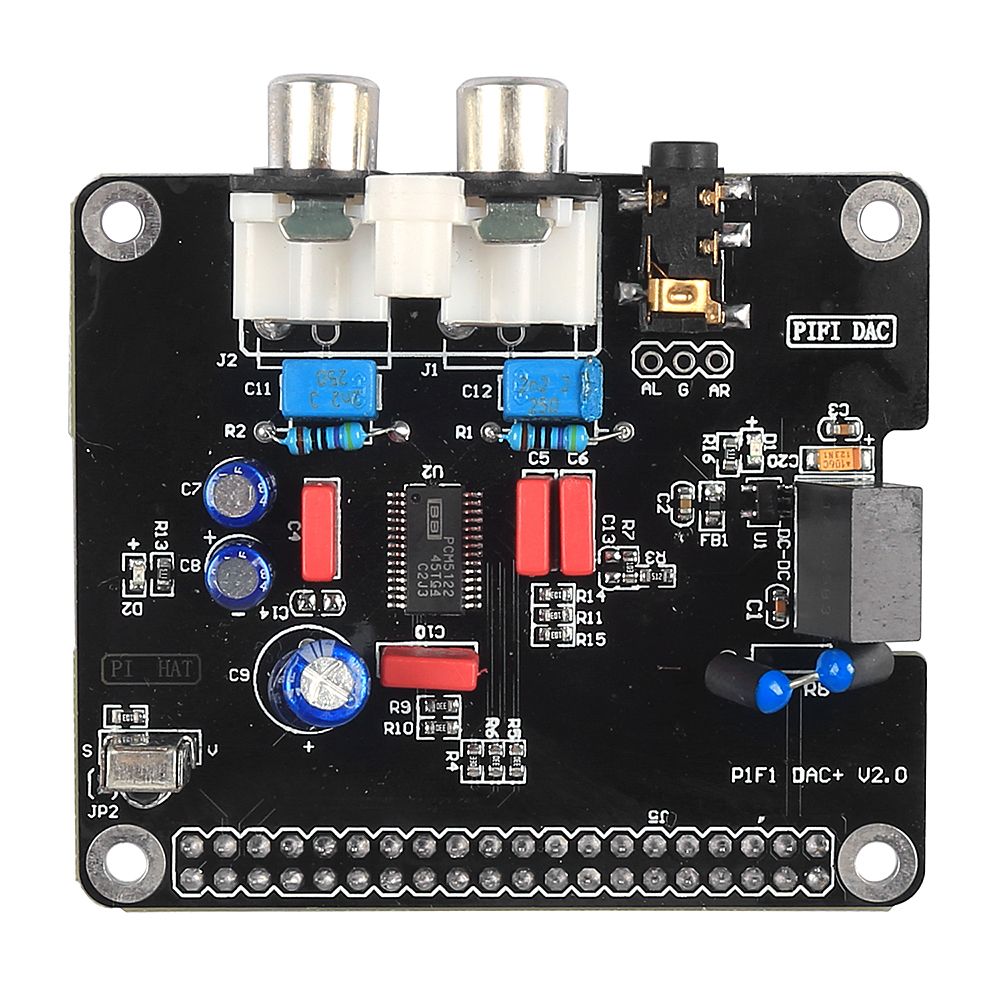
\includegraphics[width=0.5\linewidth]{./img/SainSmart_HIFI_DAC.jpeg}
	\caption{Ein \glsentryshort{i2s}-\glsentryshort{dac} mit passendem Arduino-Header \\
	\tiny\textit{Quelle: \url{https://www.sainsmart.com/sainsmart-hifi-dac-audio-sound-card-module-i2s-interface-for-raspberry-pi-2-b.html}}}
	\label{fig:sainsmarthifidac}
	\end{figure}
	
	
	\glsentryfirst{i2s} ist der Standard für die digitale Kommunikation zwischen einer Audioquelle und einem \glsentryfirst{dac}. 
	Der \gls{dac} generiert die analogen Wellen, welche in Lautsprechern Schallwellen erzeugen. Die Klangqualität ist zum größten Teil von der Qualität des \gls{dac} abhängig.
	Bei dem \gls{raspberrypi} Model B gibt es neben dem Standard-Pin-Header weitere 8 Pins von welchen 3 für \gls{i2s} genutzt werden können, wenn eine entsprechende Option im Kernel aktiviert wurde. \cite{jaekelrpidac}
	Bei neueren Modellen entsprechen die GPIO-Pins 18, 19 und 20 des Prozessors den benötigten \gls{i2s}-Pins und können einfach über den Pin-Header des \gls{raspberrypi} an den Pins 12, 35 und 38 erreicht werden. \cite{smithrpidac} Es werden auch \gls{i2s}-\gls{dac} produziert, welche einfach auf den \gls{raspberrypi} gesteckt werden können. Ein Beispiel ist in \myref{fig:sainsmarthifidac} zu sehen.
	Auch bei anderen \glspl{sbc} gibt es oft Möglichkeiten, den \gls{i2s}-BUS zu erreichen. So verfügen Beispielsweise die kostengünstigen und in vielen \gls{sbc} verwendeten Prozessoren Allwinner H3 und H5 über die entsprechenden Pins. 
	
	Bei den meisten \glspl{distribution} ist eine Unterstützung von \gls{i2s} im Kernel vorhanden. Die Pins müssen durch eine Konfiguration beim Boot aktiviert werden.
	
	Neben \gls{i2s} verfügen die meisten \gls{sbc} auch über USB-Anschlüsse. Während die Einrichtung des \gls{i2s}-Bus sich in der Software als aufwändig herausstellen kann und bei mangelnder Dokumentation die benötigten Pins nicht gefunden werden, gibt es die Alternative, einen USB-\gls{dac} zu verwenden. Diese werden einfach wie in \myref{fig:adafruitusbdac} in einen USB-Anschluss gesteckt. Die benötigten Kernelmodule sind in der Regel bereits aktiv. 
	
	Angeschlossene Audiogeräte können mit \mintinline{shell}{aplay -l} aufgelistet werden.
	
	\begin{figure}
	\centering
	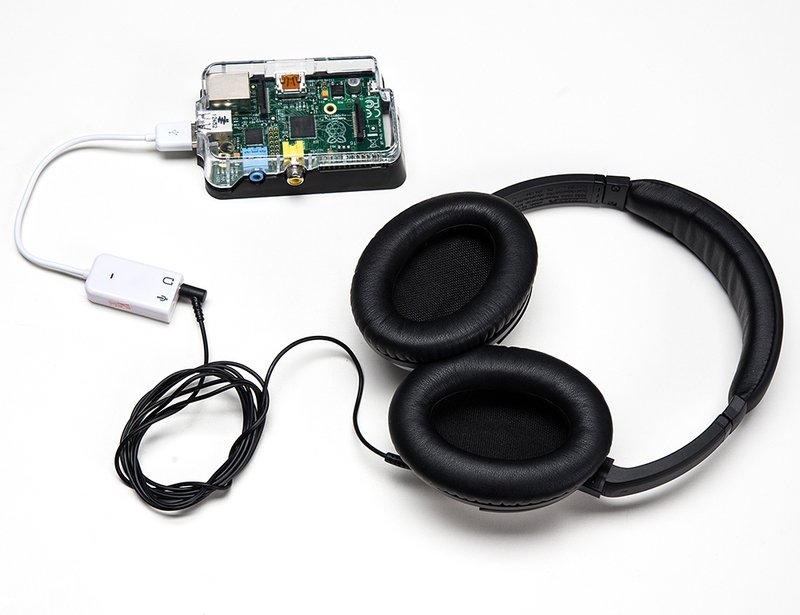
\includegraphics[width=0.5\linewidth]{./img/Adafruit_USB_DAC.jpg}
	\caption{Ein USB-\glsentryshort{dac} an einem \gls{raspberrypi} \\
	\tiny\textit{Quelle: \url{https://learn.adafruit.com/usb-audio-cards-with-a-raspberry-pi/cm108-type}}}
	\label{fig:adafruitusbdac}
	\end{figure}
	
\section{Audiowiedergabe mit Python}\label{sec:audiopython}
	Für das Abspielen von Audiodateien mit Python gibt es eine Vielzahl von Bibliotheken, jedoch keine davon hat sich als Standard etabliert. Nachfolgend werden einige dieser Bibliotheken mit Vor- und Nachteilen aufgelistet.
	
\subsection{Snack}
	Snack ist ein Toolkit für verschiedene Sprachen, welches das einfache Abspielen und Steuern von Audiowiedergaben ermöglichen soll. Es ist in C geschrieben und verfügt über viele Module die unterschiedliche Dateiformate für Musik unterstützen. \cite{snack}
	Leider ist dieses Toolkit nur mit Python bis Version 2.2 kompatibel. Da in diesem Projekt die Verwendung von Python 3 nötig war, wie in anderen Kapiteln ersichtlich wird, konnte Snack nicht verwendet werden.
	
\subsection{PyAudio}
	PyAudio bietet Zugriff auf die Funktionen der Systemweit verwendbaren PortAudio-Bibliothek. 
	PortAudio dient als Schnittstelle um Programmen den Zugriff auf die Audiohardware zu erleichtern. Der Nachteil der PyAudio-Bibliothek ist der geringe Funktionsumfang von PortAudio. So kann Theoretisch alles darüber abgespielt werden, es sind jedoch keine Decoder enthalten. Um mit PyAudio beispielsweise eine MP3-Datei abzuspielen würde ein Decoder benötigt, mit welchem die Datei eingelesen und an PortAudio übertragen werden kann. Die Recherche und Integration solcher Decoder in das Programm hätte den Rahmen dieser Arbeit weit gesprengt und wurde daher nach einigen Versuchen verworfen. \cite{pyaudio}
	
\subsection{GST-Python}\label{ssec:gst-python}
	GST-Python erlaubt Zugriff auf die von vielen Linux-Programmen verwendete GStreamer-Bibliothek. Während GStreamer sehr umfangreich ist und über eine Vielzahl von Funktionen zu verfügen scheint, konnte keine Dokumentation wie diese nun durch GST-Python zu verwenden wären, gefunden werden. Die Implementierung scheint sich nicht nach üblichen Python-Standards zu richten. Möglicherweise ist diese Bibliothek auch nur mit Pyhton 2 kompatibel, wenn auch eine Portierung einfach sein sollte.
	
\subsection{PyGame.Mixer}
	Die Pygame-Bibliothek ist eine umfangreiche Sammlung von Funktionen, welche zur Entwicklung von Spielen mit Python nötig sind. Die Verwendung des Mixer-Moduls sehr einfach. Es ist in der Lage, viele verschiedene Dateitypen zu öffnen und mit wenigen Befehlen abzuspielen. Es werden Playlists und das Abspielen mehrerer Dateien parallel unterstützt. Da es allerdings darauf ausgelegt ist, kurze Sounds in Spielen wiederzugeben, fehlen einige Funktionen, welche für einen Mediaplayer nötig sind. So ist es beispielsweise nicht möglich, die aktuelle Position im laufenden Musiktitel zu bestimmen oder allgemeine Informationen zu den Musikdateien auszulesen. Zudem ist das Mixer-Modul an die übrige PyGame-Bibliothek gebunden und kann nicht ohne diese installiert werden. Die PyGame-Bibliothek stellt, aufgrund ihres großen Umfangs, viele Anforderungen an das System. So werden für die Installation von PyGame einige Grafik-Module bis hin zu einer Denktopumgebung im Betriebssystem benötigt. Diese Anforderungen sind zu hoch, für den Betrieb auf einem \gls{headless} \gls{sbc}. \cite{pygamemixer}
	
\subsection{Steuerung anderer Mediaplayer}
	Python bietet viele Möglichkeiten, mit anderen Programmen im Betriebssystem zu interagieren. 
	So ist es einem Python-Programm möglich, andere Mediaplayer zu starten und diese entweder über die Kommandos auf der Konsolenebene, simulierte Tasteneingaben oder Socketverbindungen zu steuern.
	Dieser Ansatz wurde nach der Prüfung vieler anderer Methoden gewählt.
	Als Mediaplayer wurde der VLC-Player verwendet, da dieser über viele benutzbare Interfaces, einen großen Funktionsumfang, maximale Kompatibilität mit vielen Medienquellen und den betrieb als \enquote{VLC-noX} in \gls{headless} Systemen erlaubt. \cite{vlc-nox}
	Dabei entstand die VLC-Bibliothek, auf welche im Kapitel \ref{sec:vlclib} eingegangen wird. 
	
\section{Websockets}\label{sec:websockets}
	Herkömmliche Client-Server-Kommunikation mit JavaScript erlaubte bisher nur Anfragen vom Client an den Server. 
	In vielen Anwendungen ist dies allerdings nicht ausreichend. So mussten bisherige Webclients die Updates vom Server brauchten, wie beispielsweise in einem Chatprogramm, in regelmäßigen Abständen Anfragen an den Server stellen, um diese Updates zu erhalten. Dies erschwerte die Entwicklung von Client-Server Anwendungen mit Webtechnologien und sorgte für ineffiziente Kommunikation.
	
	Mit \glspl{websocket} ist es dem Client möglich, einen Kanal zum Server aufzubauen. Über diesen können in beide Richtungen asynchron Daten gesendet werden. Bekommt der Server zum Beispiel durch einen anderen Client ein Nachricht, so kann er alle Clients über die Neuerung informieren. Auf dem Server werden dafür alle Websocket-Verbindungen gespeichert und in jeder auf neue Nachrichten gewartet.
	
	Eine Websocket-Verbindung startet als normale HTTP-Get Anfrage. Der Header dieser Anfrage wird um \enquote{pgrade}-Argument mit dem Wert \enquote{\mintinline{text}{websocket}} erweitert.
	Der Server antwortet mit einem identischen Header und dem zusätzlichen \enquote{\mintinline{text}{Sec-WebSocket-Accept}}-Argument das als Wert einen \gls{hash} der \gls{uuid} des Clients antwortet. Der Server schließt die Übertragung an dieser stelle allerdings noch nicht ab, sondern behält die offene Verbindung, um in Zukunft darüber weitere Pakete an den Client senden zu können.
	
	Ein Datenpaket im Websocket hat wiederum einen eigenen Header, welcher mit Hilfe einer Maske der Unterscheidung zwischen Server- und Client-Paketen ermöglicht. Der Server maskiert dabei kein Paket, währen der Client alle Pakete maskieren muss. Für die Maskierung wird auf alle Daten im Paket ein \gls{xor} mit einer Maske im Header des Pakets angewendet. \cite{rfc6455}
	
	Da die Verbindungen offen bleiben, muss Serverseitig beachtet werden, dass Verbindungen asynchron bearbeitet werden. 
	Bei einer einfachen synchronen Verarbeitung von anfragen, kann ein Server immer nur eine Anfrage zu einem bestimmten Zeitpunkt bearbeiten. Da Websockets als normale HTTP-Anfragen zählen, die allerdings erst bei schließen der Verbindung durch den Client beendet werden, würde es dazu kommen, dass, während ein Client verbunden ist, kein anderer eine Verbindung aufbauen kann. Wie dieses Problem mit Hilfe von Asyncio und AIOHTTP in Pyhton gelöst werden kann, wird in Abschnitt \ref{sec:py36} beschrieben.
	
	
\section{Python 3.6, Asyncio und AIOHTTP}\label{sec:py36}
	Python bietet seit Version 3.4 die Asyncio-Standardbibliothek  an. Damit ist es möglich, asynchrone, nebenläufige Koroutinen zu implementieren. Im Gegensatz zu sequentieller Programmierung von Aufgaben werden asynchrone Aufgaben gleichzeitig ausgeführt. Dies ermöglicht die Trennung verschiedener Aufgaben voneinander, welche gleichzeitig ausgeführt werden müssen. Verglichen mit Parallelen Prozessen, werden dafür nicht mehrere Prozessoren benötigt.  
	Ein Vorteil von nebenläufigen Prozessen über parallelen Prozessen ist, dass die Kommunikation zwischen Prozessen sowie das Teilen von gemeinsamen Ressourcen deutlich einfacher möglich ist. Bei parallelen Prozessen muss darauf geachtet werden, dass nie 2 Prozesse gleichzeitig auf gemeinsam genutzte Daten zugreifen. Dafür werden Sperren eingesetzt, welche ein Prozess nutzen kann, um andere Prozesse an der Benutzung einer Variable zu hindern, während die vom ersten Prozess verwendet wird. Da bei nebenläufigen Koroutinen immer nur eine Routine zu einem bestimmten Zeitpunkt arbeitet, kann sichergestellt werden, dass nur diese in einem Moment Zugriff auf alle Daten hat. 
	
	Dafür wird von einem Prozess-Scheduler immer abwechselnd jeweils einem Prozess die Möglichkeit zur Ausführung gegeben. Dieser muss, wenn er eine Teilaufgabe erledigt hat, die Kontrolle zurück zum Scheduler geben, damit der diese einem anderen Prozess zuweisen kann. Die größte Gefahr die bei der Entwicklung mit Koroutinen besteht darin, dass eine Routine nie die Kontrolle dem Scheduler zurück gibt.
	
	
	\begin{figure}[h]
		\centering
		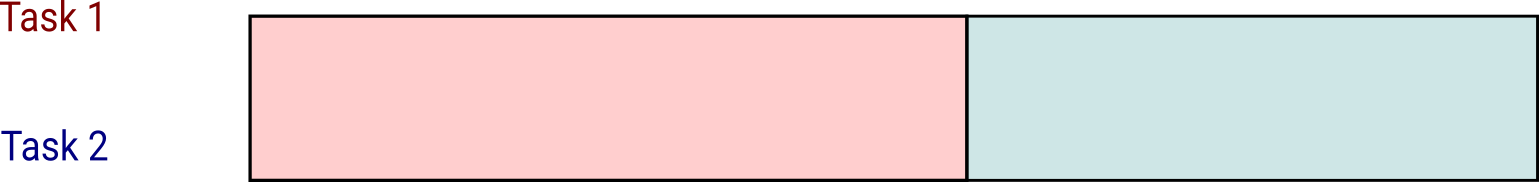
\includegraphics[width=0.7\linewidth]{./img/sequenziell.png}
		\caption{sequentielle Ausführung von Prozessen}
		\label{fig:sequenziell}
	\end{figure}
	
	\begin{figure}[h]
		\centering
		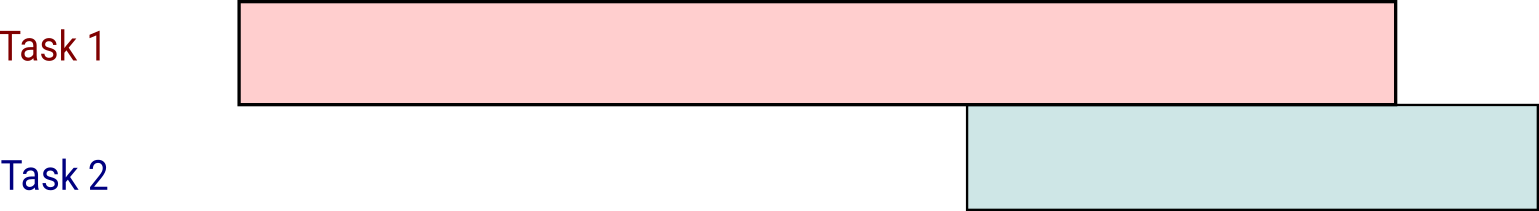
\includegraphics[width=0.7\linewidth]{./img/parallel.png}
		\caption{parallele Ausführung von Prozessen}
		\label{fig:parallel}
	\end{figure}
			
	\begin{figure}[h]
		\centering
		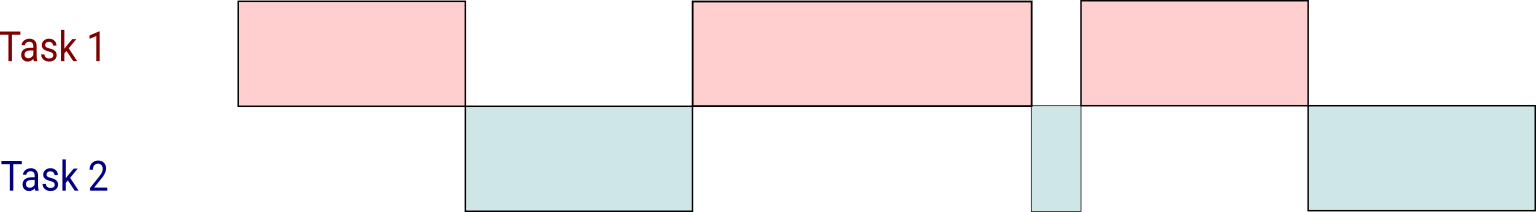
\includegraphics[width=0.7\linewidth]{./img/concurrent.png}
		\caption{nebenläufig, asynchrone Ausführung von Prozessen}
		\label{fig:concurrent}
	\end{figure}
	
	
	Asyncio wurde speziell mit dem Hintergedanken der gleichzeitigen Verarbeitung mehrerer Ein- und Ausgaben entwickelt. So ist es einem Prozess möglich, auf eine neue Eingabe zu warten. Der Scheduler weist der Wertenden Koroutine nie die Konrtolle zu, bis die erwartete Eingabe erfolgt. So können effizient andere Aufgaben erfüllt werden, während die Koroutine auf eine Eingabe wartet.
		
	In Python wird eine Koroutine durch das Schlüsselwort \mintinline{python3}{async} vor der normalen Methodendefinition gekennzeichnet. Durch den Befehl \mintinline{python3}{yield} wird die Kontrolle an den Scheduler zurück gegeben. An dieser Stelle wird die Methode weiter ausgeführt, sobald der Scheduler ihr in Zukunft die Kontrolle zurück gibt.
	Mit dem Befehl \mintinline{python3}{await} und einer weiteren Koroutine, übergibt die erste Koroutine einer anderen die Kontrolle und wartet darauf, dass diese abgeschlossen wird. Bis zu dem Abschluss kann die untere Koroutine die Kontrolle an den Scheduler zurück geben und tritt allgemein an die stelle der ausführenden Koroutine. Ruft die untere Koroutine während der Ausführung \mintinline{python3}{yield} mit einem Wert auf, so ist es möglich, in der oberen diesen asynchron zu verarbeiten.

	\begin{sourcecode}[h]
	\caption{Beispiel einer Asyncio Koroutine}
	\label{fig:asyncio-example}
	\begin{mycode}{python3}
async def koroutine(self):
	print("Koroutine gestartet")
	# gebe erstmals die Kontrolle zum Scheduler zurück
	yield	
	while True:
		print("Koroutine läuft")
		# Gebe die Kontrolle an den Scheduler zurück
		#  und warte auf den Abschluss der in asyncio
		#  vordefinierten sleep-Koroutine.
		# Sleep wartet n=5 Sekunden.
		await asyncio.sleep(5)

	\end{mycode}
	\end{sourcecode}
		%In \codepageref{fig:imagepreview-html5example} ...\\
\subsection{AIOHTTP}
	AIOHTTP ist enthält Implementierung verschiedener \gls{http}-Clients und -Server, welche mit Asyncio kompatibel sind. So können Anfragen asynchron verarbeitet werden, was die gleichzeitige Benutzung eines Servers durch mehrere Clients oder die Bereitstellung mehrerer Server erlaubt. Auch eine Implementierung des WebSocket-Protokolls ist enthalten. Speziell für dieses ist die asynchrone Ausführung wichtig, wie in Abschnitt \ref{sec:websockets} erklärt wurde.


\chapter{Umsetzung}\label{ch:umsetzung}
	Für die Umsetzung wurde zunächst eine Bibliothek zur Steuerung des VLC-Mediaplayers implementiert. 
	Diese wird von der Implementierung des Websocket-Servers benutzt, welcher einen Websocket bereit stellt, über welchen wiederum der Mediaplayer gesteuert werden kann. Theoretisch wäre es möglich die Bibliothek zur Steuerung des VLC-Mediaplayers durch eine andere mit ähnlicher Funktionalität zu ersetzen, um andere Mediaplayer oder eine eigene, python-basierte Implementierung zum Abspielen von Audiodateien über den Websocket zu steuern.
	Bei der Implementierung des Websocket-Servers wird ausgenutzt, dass AIOHTTP mehrere Prozesse gleichzeitig ausführen kann (siehe Abschnitt \ref{sec:py36}) und Websockets auf normalen HTTP-Get-Anfragen basieren (siehe Abschnitt \ref{sec:websockets}) um neben dem Websocket auch die für den Webclient benötigten Dateien bereitszustellen.
	Der Webclient ist in modernem HTML5 mit HTML-Imports umgesetzt und baut eine Verbindung zum Websocket auf, über welchen er Updates des Players erhält und Nutzereingaben an den Server überträgt.
	In Abbildung \ref{fig:conectionsoverview} wird zur Verdeutlichung der Verbindungen ein Ablauf mit zwei Clients dargestellt. In der Abbildung wird nur die Position im aktuellen Titel betrachtet. In der Praxis wären neben der Position auch äquivalente Abläufe für andere Elemente, wie die Playliste, den aktuellen Titel oder das aktuelle Albumbild nötig.
	
	Der Mehrwert des asynchronen Websockets und des neuen Webfrontends gegenüber der HTTP-Schnittstelle und dem Webfrontend des VLC-Players besteht darin, dass diese Implementierung asynchron arbeitet.
	Das Webfrontend des VLC-Players kann nicht von mehreren Nutzern gleichzeitig fehlerfrei genutzt werden. Die Implementierung dieses Websockets ermöglicht die Bündelung der Anfragen mehrerer Nutzer, leitet diese an den sequentiell arbeitenden HTTP-Server des VLC-Players weiter und informiert alle Nutzer des Websockets asynchron über Neuerungen am Player.
	\newpage
	\begin{figure}[H]
	\centering
	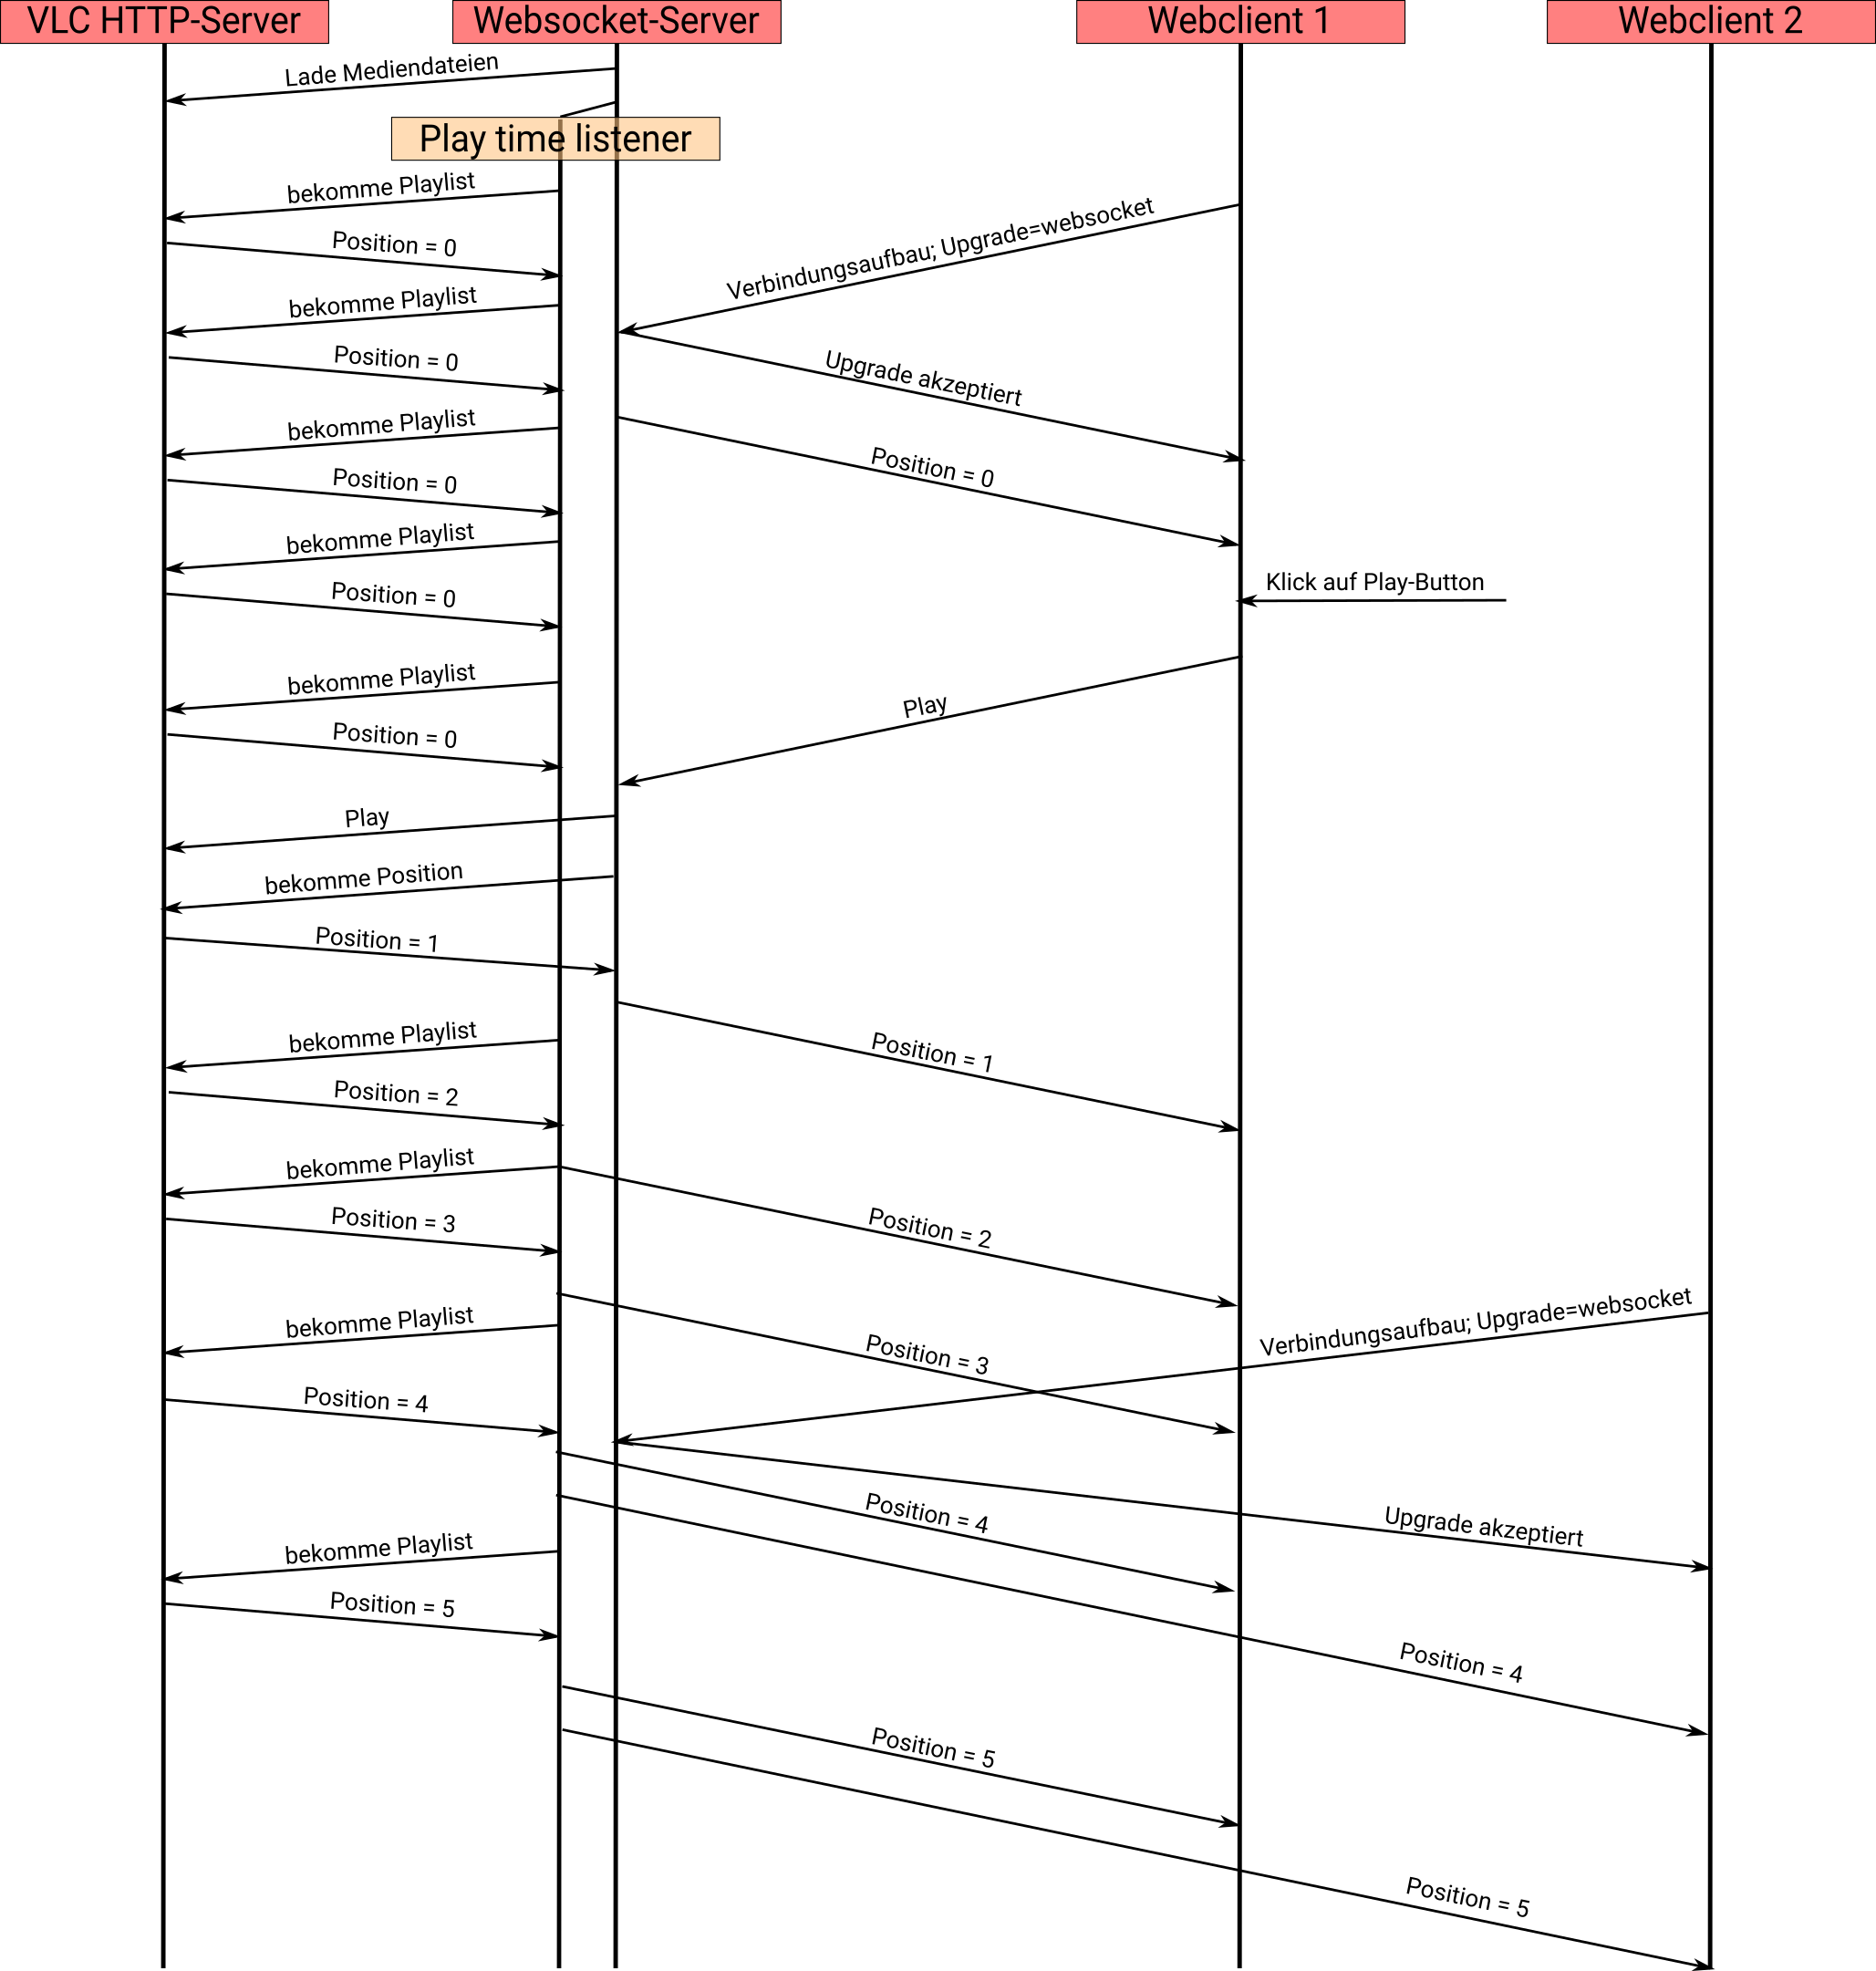
\includegraphics[width=\linewidth]{img/conections_overview}
	\caption{Sequenzdiagram der Verbindungen von zwei Clients mit dem Websocket}
	\label{fig:conectionsoverview}
	\end{figure}
	\newpage
	

\section{VLC-Bibliothek}\label{sec:vlclib}
	Die VLC-Bibliothek prüft beim Ausführen, ob bereits eine Instanz des VLC-Players ausgeführt wird. Ist dies nicht der Fall, so startet sie den VLC-Mediaplayer mithilfe der seit Python 3.0 vorhandenen subprocess-Bibliothek in einem externen Prozess aus. Der VLC-Player wird in einem Linux-Screen (virtuelle Konsolensitzung) ausgeführt. Dies hat den Vorteil, dass bei Neustart des Servers der bereits laufende VLC-Prozess einfacher wiedergefunden werden kann. Ein Nachteil ist allerdings, dass diese Methode nur unter Linux funktioniert. Wird der VLC-Player bereits ausgeführt, so wird lediglich eine Verbindung zu diesem aufgebaut.
	
	Diese Bibliothek hat starke Einflüsse durch ein von Marios Zindilis entwickeltes Skript zur Kontrolle des VLC-Players von. Das ursprüngliche Skript war für die Benutzung in Python 2 geschrieben und konnte den VLC-Player nur über das RC-Interface steuern. Auch bei dieser Steuerung gab es erhebliche Probleme, da kaum Buffering betrieben wurde und viele Funktionen, welche vom VLC-Player angeboten werden, nicht genutzt wurden. \cite{vlcpython}
	Das ursprüngliche Skript wird durch das neue Skript um mehr Möglichkeiten beim Starten des VLC-Players, der Unterstützung des HTTP-Interfaces sowie ein überarbeitetes Buffering der Antworten des VLC-Players erweitert und im Python 3 implementiert.
	
	Der Verbindungsaufbau zum VLC-Player ist momentan nur über das RC- und das HTTP-Interface möglich. Das RC-Interface wird momentan noch nicht vollständig von dieser Bibliothek unterstützt. Daher ist eine Verbindung über das HTTP-Interface zu empfehlen.
	
	Das RC-Interface des VLC-Players ist auf die Benutzung durch eine Kommandozeile und für Verbindungen zum RC-Socket über ein Netzwerk vorgesehen. Wird das RC-Interface verwendet, so baut die VLC-Bibliothek bei Initialisierung eines VLC-Objektes eine Verbindung zu dem Socket auf. Dafür wird die in Python vorhandene Socket-Bibliothek verwendet. 
	Nach dem Verbindungsaufbau können Befehle an den Socket gesendet werden. Anschließend kann durch das Auslesen des Socketbuffers die Antwort des VLC-Players bestimmt und für die Benutzung in Pyhton passend formatiert werden.
	Die verwendbaren Befehle können eingesehen werden, indem der VLC-Player auf der Kommandozeile mit dem RC-Interface ausgeführt wird und der Help-Befehl eingegeben wird. Alle wichtigen Befehle werden in der Bibliothek durch Methoden wiedergegeben. Der Anwender der VLC-Python-Klasse braucht kein weiteres Wissen über die verwendeten Kommandos.
	
	Die Verbindung zum HTTP-Interface erfolgt über die Requests-Bibliothek. Es werden normale HTTP-Get-Anfragen an die HTTP-Schnittstelle des VLC-Players gestellt. Die Antworten werden im JSON-Format geladen und automatisch in Python-Objekte umgewandelt. Eine Dokumentation der möglichen Anfragen und zu erwartenden Antworten kann in den Dateien des VLC-Players gefunden werden. Auch in dem Repository des Quellcodes des VLC-Players sind sie vorhanden. \cite{vlchttpdoc}
	
	Unabhängig davon, welches Interface beim Laden des VLC-Objektes gewählt wurde, können alle funktionen ausgeführt werden. Diese werden intern an das zu verwendende Interface weitergeleitet.
	
	Der Code der VLC-Bibliothek kann in der Datei \mintinline{text}{vlc.py} im Ordner \mintinline{text}{vlc} eingesehen werden.
	
\section{Asynchroner Websocket-Server in Python}
	Das Server-Skript startet zu Beginn einen Asynchronen Server der AIOHTTP-Bibliothek und führt zusätzlich eine Liste von Koroutinen aus, die jeweils in bestimmten Abständen über die VLC-Bibliothek Anfragen an den VLC-Player stellen um Informationen von diesem zu erhalten. Da der VLC-Player keine Asynchrone Verbindung anbietet, ist nur dieses regelmäßige Überprüfen möglich. 
	
	Dies ist auch ein Grund für die Implementierung des Websockets, da ohne diesen das bereits vorhandene Webfrontend des VLC-Players nicht Asynchron funktioniert. Durch die regelmäßigen Anfragen des Websocket-Servers an den VLC-HTTP-Server und das anschließend asynchrone Verteilen an alle Clients wird aus dem synchronen Single-User-System ein asynchrones System, welches mehrere Nutzer erlaubt.
	
	Der zu Beginn gestartete AIOHTTP-Server prüft bei jeder Anfrage, ob diese ein Upgrade zum Websocket anfordert (siehe Abschnitt \ref{sec:websockets}. 
	Wird kein Upgrade der Verbindung gefordert, werden die Dateien eines Unterverzeichnisses bereitgestellt, welche vom Browser des Nutzers geladen und als Webclient ausgeführt werden können (siehe Abschnitt \ref{sec:webclient}). 
	
	Wird ein Upgrade zum Websocket gefordert, so wird die Anfrage mit dem Websocket-Header beantwortet und die Koroutine am Leben erhalten, bis die Verbindung vom Client geschlossen wird. Die offenen Websocket-Verbindungen werden in einer gemeinsamen Liste gespeichert, um den Zugriff durch andere Koroutinen zu erlauben. Bei Verbindungsabbau werden die Verbindungen aus der Liste gelöscht.
	Bei eingehenden Anfragen durch den Websocket werden diese in einer \mintinline{python3}{on_ws_message}-Methode interpretiert und auf Befehle an das VLC-Objekt umgesetzt. Neuerungen am VLC-Objekt werden anschließend an alle verbundenen Clients übertragen.

	Der Quellcode des Servers befindet sich in der Datei \mintinline{text}{serve.py} im Hauptordner des Projekts. Diese Datei muss gestartet werden, um das gesamte Projekt auszuführen. Sie Erlaubt das Anhängen von Parametern wie die Position der Abzuspielenden Mediendateien oder der vom Server zu verwendenden Ports.

\newpage
\section{Webclient}\label{sec:webclient}
	Der Webclient besteht aus 3 Modulen. Diese werden mit Hilfe von HTML-Imports miteinander verbunden. HTML-Imports erlauben eine Objektorientierte Strukturierung von HTML5-Projekten. Dabei wird in jedem Modul der benötigte HTML-Code in einem Template gespeichert und mit dazu gehörigem Javascript geladen und ausgeführt. \cite{w3c-customEm-0216}
	Ein Beispiel für ein selbst definiertes HTML-Element in einer Datei, welche importiert werden kann ist im Quellcode \ref{fig:custom-element-example} auf Seite \pageref{fig:custom-element-example} zu sehen.
	Dabei werden eigene HTML-Tags definiert, welche mit \mintinline{html}{<link rel="import" href="Quelle.html"/>} in anderen HTML-Modulen geladen und anschließend als eigener HTML-Tag in die Seite eingefügt werden können.
	
	Das Webfrontend basiert auf HTML-Code von Uğur Oruç und wurde restrukturiert sowie durch Funktionalität im JavaScript ergänzt. \cite{materializemusic}
	
	\begin{figure}
	\centering
	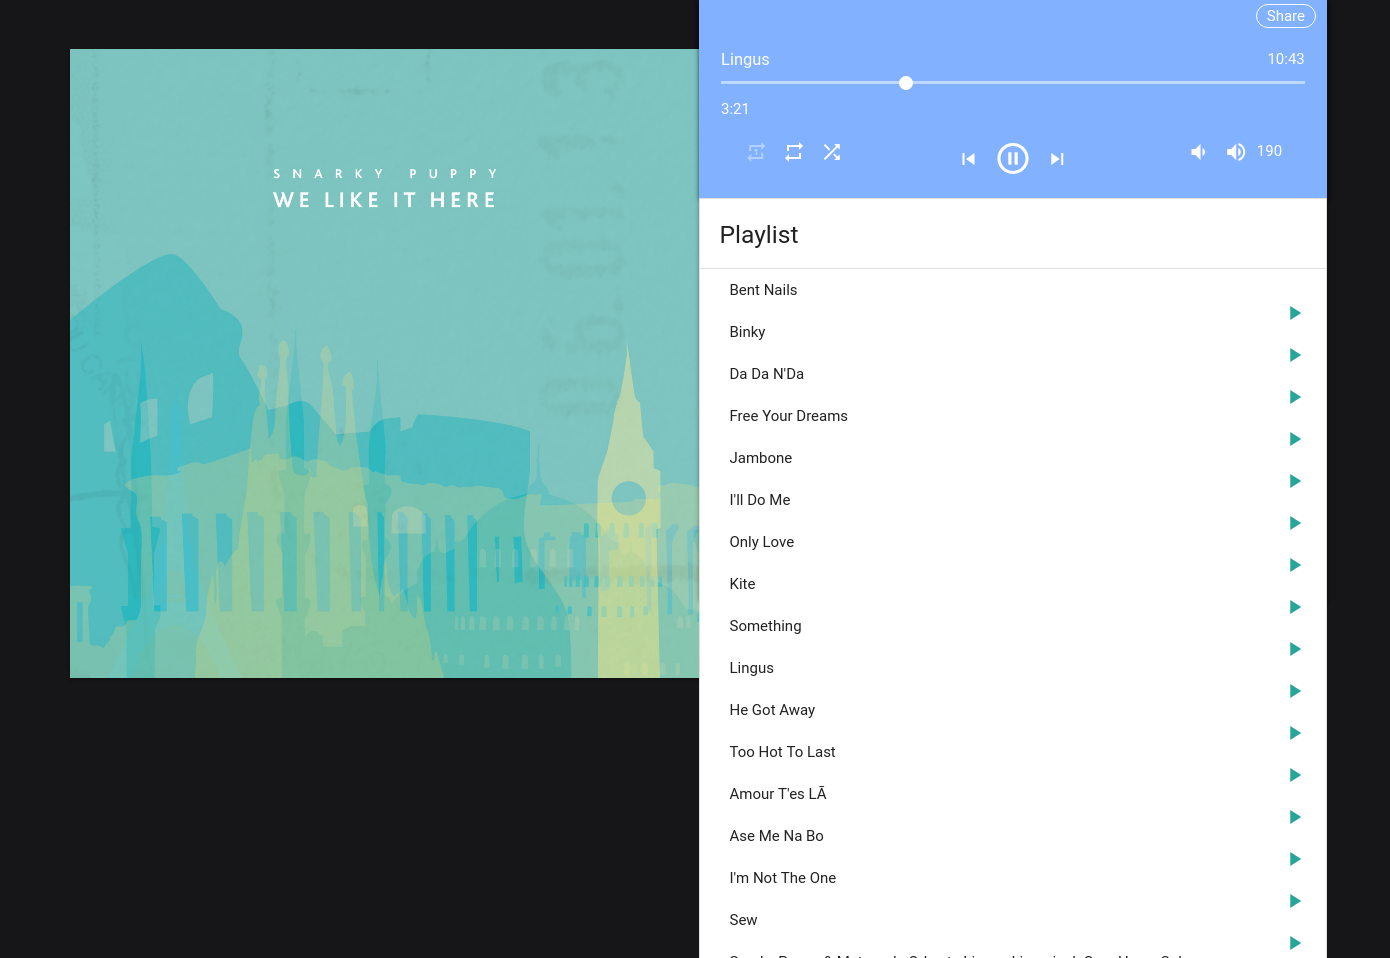
\includegraphics[width=0.8\linewidth]{./img/Screenshot_20170717_211638.png}
	\caption{Ansicht des Webfrontends}
	\label{fig:screenshot20170717211638}
	\end{figure}
	
	Das Hauptelement des Webclients stellt eine Verbindung zum Websocket her und zeigt dem Nutzer alle Steuerungselemente. 
	Es implementiert die Funktionalität dieser Elemente und sendet bei Nutzereingaben Befehle über den Websocket an den Server. Bei eingehenden Befehlen vom Server werden diese auf die damit verbundenen Elemente in der HTML-Seite angewendet.
	
	Das Hauptelement \mintinline{html}{<music-app>} läd die Definition des \mintinline{html}{<song-list>}-Elements und legt eine Instanz davon an. Dem \mintinline{html}{<song-list>}-Element wird beim empfangen einer neuen Playlist vom Server diese zusammen mit dem Template einer Funktion zum Wechseln des aktuellen Titels übergeben.
	Im \mintinline{html}{<song-list>}-Element wird für jeden Titel in der Playlist ein \mintinline{html}{<song-entry>}-Element angelegt. Diesem wird die passende Funktion zum wechseln des Titels übergeben. Wird ein Button im \mintinline{html}{<song-list>}-Element angeklickt, so kann dieses die Funktion ausführen und der Titel wird gewechselt.
	
	Der Quellcode des Webclients befindet sich im Unterordner \mintinline{text}{webclient}. Es ist zu beachten, dass dieser in einigen Browsern, inklusive dem Internet Explorer von Microsoft sowie in Firefox angezeigt wird. Diese Browser unterstützen das neue Konzept der HTML-Imports aktuell noch nicht. Die Funktion des Webclients wurde bisher nur in der aktuellen stabilen Version des Chromium-Browsers unter Linux und Android getestet.
	

	\begin{sourcecode}[h]
	\caption{Beispiel eines eigenen HTML-Elements, welches als Import geladen werden kann}
	\label{fig:custom-element-example}
	\begin{mycode}{html}
<!DOCTYPE html>
<template id="halloWeltTemplate">
	<div><i>Hallo Welt!</i></div>
</template>
<script>
	var HalloWeltProto = Object.create(HTMLElement.prototype);
	HalloWeltProto.ownerDoc = document.currentScript.ownerDocument;

	HalloWeltProto.createdCallback = function () {
		// get reference to main document
		var template = this.ownerDoc.querySelector('#halloWeltTemplate');
		var instanceClone = document.importNode(template.content, true);
		this.appendChild(instanceClone);
	};
	HalloWeltProto.attachedCallback = function () {
		// Wird ausgeführt, wenn das Element dargestellt wird
	};
	HalloWeltProto.detachedCallback = function () {
		// Wird ausgeführt, wenn das Element entfernt wurde
	};
	HalloWeltProto.attributeChangedCallback = function (attrName, oldVal, newVal) {
		// Wird ausgeführt, wenn sich ein Attribut des Elements ändert
	};
	var HalloWelt = document.registerElement('hallo-welt', {prototype: HalloWeltProto});
	// Das Element kann jetzt als <hallo-welt></hallo-welt> eingefügt werden.
</script>
	\end{mycode}
	\end{sourcecode}

\chapter{Installation}\label{ch:installation}
	Zu den Bedingungen zählen zunächst der VLC-Player oder für den Betrieb auf einem \gls{headless} Computer VLC-noX.
	Außerdem wird Python 3.6 benötigt.
	Die Installation der Abhängigkeiten in Debian basierten Systemen, wie Raspbian oder Armbian mit folgendem Befehl möglich:
	\\
	\begin{mycode}{sh}
sudo apt-get install vlc-nox python36
	\end{mycode}
	\\
	Optional kann auch \mintinline{sh}{git} über \mintinline{sh}{apt-get} installiert werden, um später den Quellcode des Projekts von Github zu laden.
	
	Anschließend müssen einige Abhängigkeiten in Python installiert werden. Hierfür kann \mintinline{sh}{pip} verwendet werden. Sind mehrere Versionen von Python installiert und Python 3.6 ist nicht als Standardversion gewählt, muss der Befehl \mintinline{sh}{pip3.6} benutzt werden. In diesem Fall bietet sich auch an, eine virtuelle Umgebung für Python 3.6 anzulegen und in diese zu wechseln.
	\\
	\begin{mycode}{sh}
(sudo) pip install requests aiohttp
	\end{mycode} 
	\\
	
	Ist der Quellcode des Projekts noch nicht vorhanden, so kann er über Git geladen werden:
	\\
	\begin{mycode}{sh}
git clone --recursive https://github.com/Anaeijon/Monty_Mumup.git
	\end{mycode}
	\\
	Das Argument \mintinline{sh}{--recursive} ist dabei wichtig, um alle verwendeten Submodule automatisch zu laden.
	
	Im Hauptordner des Projekts kann jetzt das \mintinline{sh}{serve.py}-Script ausgeführt werden. Es benötigt einen Ordner als Parameter, in welchem nach Musik gesucht werden soll.
	\\
	\begin{mycode}{sh}
python ./serve.py ~/Pfad/zu/Musik
	\end{mycode}
	\\
	Anschließend wer Webclient über den Port 8000 erreichbar.
	
	Das Projekt bietet auch die Möglichkeit, einen anderen Port über das Argument \mintinline{sh}{--recursive} anzugeben. Um von anderen Geräten aus auf den Server zugreifen zu können, wird empfohlen, Port 80 zu verwenden. Da in den meisten Linux-Systemen die Benutzung dieses Ports dem Superuser \mintinline{sh}{root} vorbehalten ist, muss der Server mit  \mintinline{sh}{sudo} ausgeführt werden. Da der VLC-Player allerdings nicht vom \mintinline{sh}{root} ausgeführt werden darf, muss er zuvor separat vom Nutzer gestartet werden.
	\\
	\begin{mycode}{sh}
screen -dmS vlc_screen vlc --intf http --http-host localhost --http-port 8080 \
                       --http-password pass
sudo python ./serve.py --port 80 --vlc-screen None --vlc-port 8080 --vlc-password pass
	\end{mycode}
	\\
	Mit dem Argument \mintinline{sh}{--extraintf} können weitere Interfaces zu VLC hinzugefügt werden.
%	\mintinline{sh}{ncurses} bietet sich für die Bedienung über ssh an. Über das zusätzliche Interface können weitere Titel zu VLC hinzugefügt werden.
	
	
\chapter{Ausblick}\label{ch:ausblick}

\section{Fehler und Probleme}
	Aktuell kann es in der Kommunikation mit dem VLC-Player zu Fehlern kommen. Probleme mit dem Buffering der Antworten aus dem RC-Interface sind bekannt. Daher wird bevorzugt das HTTP-Interface verwendet. Doch auch im HTTP-Interface kommt es dazu, dass der VLC-Player teilweise veraltete Informationen sendet.
	
	Einige Funktionen des Webfrontends, wie das Ändern der Position im Titel mit dem Slider-Element können dafür sorgen, dass viele Befehle gleichzeitig übertragen werden. Es kommt dadurch zu einem Stau im Websocket-Server, welcher diese an den VLC-Player weiterleiten soll. Dadurch kann es zu großen Latenzen zwischen Nutzereingabe und Reaktion des Servers kommen.

\section{Erweiterbarkeit}
	Es ist möglich, das verwendete VLC-Modul zu ersetzen. Da im Hauptprogramm keine VLC-Spezifischen Funktionen genutzt werden, kann an dieser Stelle auch ein anderer Medienplayer eingesetzt werden. Dieser muss nur die Grundfunktionen, welche vom Webfrontend angeboten werden, wie Play, Pause, Nächster Titel und weitere bereitstellen und durch eine Klasse in Python gesteuert werden. Auch eine eigene Implementierung einer Medienplayer-Klasse in Pytho, beispielsweise auf Basis der GStreamer-Bibliothek (siehe Abschnitt \ref{ssec:gst-python}) wäre möglich. 
	
	Die eigene Bibliothek zur Steuerung des VLC-Players ist nicht mit Asyncio entwickelt wurden. Dadurch kann es zu Latenzen während der Kommunikation mit dem VLC-Player kommen. Um dies zu vermeiden, müssten die verwendeten HTTP-Get-Anfragen aus der Requests-Bibliothek durch entsprechende Anfragen aus der AIOHTTP-Bibliothek ersetzt und alle Methoden der VLC-Bibliothek zu Koroutinen erweitert werden. Aktuell ist ein Vorteil der sequentiellen Implementierung der Anfragen an den VLC-Player, dass nicht sicher gestellt werden kann, ob dieser in der Lage ist, auf asynchrone Anfragen korrekt zu reagieren.
	
	Die Python-Implementierung dieses Websockets würde Obsolet werden, wenn der VLC-Player neben dem HTTP-Interface auch noch um ein Websocket-Interface erweitert würde. Die Implementierung müsste in Lua oder C geschehen.
	
	Aktuell kann nur beim Start des Servers ein Ordner angegeben werden, welcher vom Player geladen und als Playlist angezeigt wird. Es ist nicht möglich, weitere Titel hinzuzufügen. Diese Funktion sowie das Wechseln zwischen verschiedenen vordefinierten Playlists sollte in Zukuft über das Webfrontend verfügbar gemacht werden. Bis dahin kann der VLC-Player neben dem HTTP-Interface mit einem zusätzlichen Interface wie \enquote{ncurses} oder \enquote{telnet} ausgeführt werden, über welche ein Administrator weitere Titel zur Medienliste hinzufügen kann.

\section{Fazit}
	Auch wenn der verwendete VLC-Player bereits über ein eigenes Webfrontend verfügt, so bietet diese Implementierung einen Mehrwert. Nicht nur das Design sondern auch das Konzept der Client-Server-Kommunikation über Websockets ist dem alten Überlegen. Gerade bei der Benutzung durch mehrere Nutzer oder von mehreren Interfaces kommt es seltener zu Fehlern im Webclient.
	
	Bei der Entwicklung sind der Webclient und die VLC-Bibliothek als eigenständige Module entstanden, welche auch in anderen Projekten verwendet werden können.

%\chapter{Glossar}

\printglossaries
%\chapter{Anhang}

\begin{thebibliography}{99}

\bibitem{materializemusic}
	Uğur Oruç: \textbf{\textit{Materialize-Music-Player}} \\
	Quelcode: \url{https://github.com/Ketcap/Materialize-Music-Player}

\bibitem{vlcpython}
	Marios Zindilis: \textbf{\textit{Control VLC with Python}}
	\\\url{https://zindilis.com/blog/2016/10/23/control-vlc-with-python.html}
	
\bibitem{python3}
	J. Ernesti, P. Kaiser: \textit{\textbf{Python 3 : das umfassende Handbuch}}
	\\4., aktualisierte und erweiterte Auflage 2015, 1., korrigierter Nachdruck 2016
	\\Bonn : Rheinwerk Verlag, 2016

\bibitem{rfc6455}
	I. Fette, A. Melnikov: \textbf{\textsl{RFC 6455 : The WebSocket Protocol}}.
	\\Internet Engineering Task Force (IETF), December 2011 %, abgerufen am 20.03.2017 (englisch).
	\\\url{https://tools.ietf.org/html/rfc6455}

\bibitem{w3c-html5}
	W3C: \textit{\textbf{HTML5, A vocabulary and associated APIs for HTML and XHTML}}.
	\\W3C Recommendation 28 October 2014
	\\\url{https://www.w3.org/TR/html5/}

\bibitem{w3c-customEm-0216}
	W3C: \textit{\textbf{Custom Elements}}.
	\\W3C Working Draft 26 February 2016
	\\\url{https://www.w3.org/TR/2016/WD-custom-elements-20160226/}

\bibitem{docsPython36}
	%Guido van Rossum: \textsl{\textbf{Dokumentation Python} 3.0}.
	Python Software Foundation: \textit{\textbf{Python Language Reference}, Version 3.6.1}.
	%\\Python Software Foundation, 14. Februar 2009, abgerufen am 20.03.2017 (englisch).
	\\\url{https://docs.python.org/3.6/}

\bibitem{docsPython36asyncio}
	%Guido van Rossum: \textsl{\textbf{Dokumentation Python} 3.0}.
	Python Software Foundation:
	\\\textit{\textbf{asyncio — Asynchronous I/O, event loop, coroutines and tasks}, Version 3.6.1}.
	%\\Python Software Foundation, 14. Februar 2009, abgerufen am 20.03.2017 (englisch).
	\\\url{	https://docs.python.org/3/library/asyncio.html}

\bibitem{jaekelrpidac}
	Torsten Jaekel: \textbf{\textit{Audiophile, High Quality RPi-DAC for Raspberry Pi}}
	\\\url{http://www.tjaekel.com/T-DAC/raspi.html}
	
\bibitem{smithrpidac}
	Daniel Smith: \textbf{\textit{I2S Audio DAC + Amp for Raspberry Pi 2 / B+}}
	\\\url{http://www.pagemac.com/projects/i2s_amp}
	
\bibitem{snack}
	Kåre Sjölander: \textbf{\textit{The Snack Sound Toolkit}}
	\\\url{http://www.speech.kth.se/snack/}
	
\bibitem{pyaudio}
	\textbf{\textit{PyAudio Documentation}}
	\\\url{http://people.csail.mit.edu/hubert/pyaudio/docs/}
	
\bibitem{pygamemixer}
	\textbf{\textit{Pygame documentation - pygame.mixer}}
	\\\url{https://www.pygame.org/docs/ref/mixer.html}
	
\bibitem{vlc-nox}
	\textbf{\textit{vlc-noX: VLC: VideoLAN Client - without X dependencies}}
	\\\url{https://download.videolan.org/vlc/0.8.6/SuSE/11.1/repodata/repoview/vlc-noX-0-1.1.2-2.9.html}
	
\bibitem{vlchttpdoc}
	\textbf{\textit{VLC http requests README.txt}}
	\\\url{https://github.com/videolan/vlc/blob/master/share/lua/http/requests/README.txt}
	
\end{thebibliography}
%\newpage
%\chapter{Eigenständigkeitserklärung}
%Hiermit versichere ich, dass ich die vorliegende Arbeit „Entwicklung von Steuerung und Komponenten für Live Escape Games” %bisher bei keiner anderen Prüfungsbehörde eingereicht,
%sie selbstständig verfasst und keine anderen als die angegebenen Quellen und
%Hilfsmittel benutzt sowie Zitate kenntlich gemacht habe.
%\\\\\par
%\begin{tabular}{lp{2em}l}
% \hspace{5cm}   && \hspace{4cm} \\\cline{1-1}\cline{3-3}
% Ort, Datum     && Unterschrift
%\end{tabular}


%\chapter{Verzeichnisse}
%\lstlistoflistings

\end{document}
